% 2. Paper methodology
\section{Paper methodology}


\begin{frame}{Batch vs Instance Normalization}
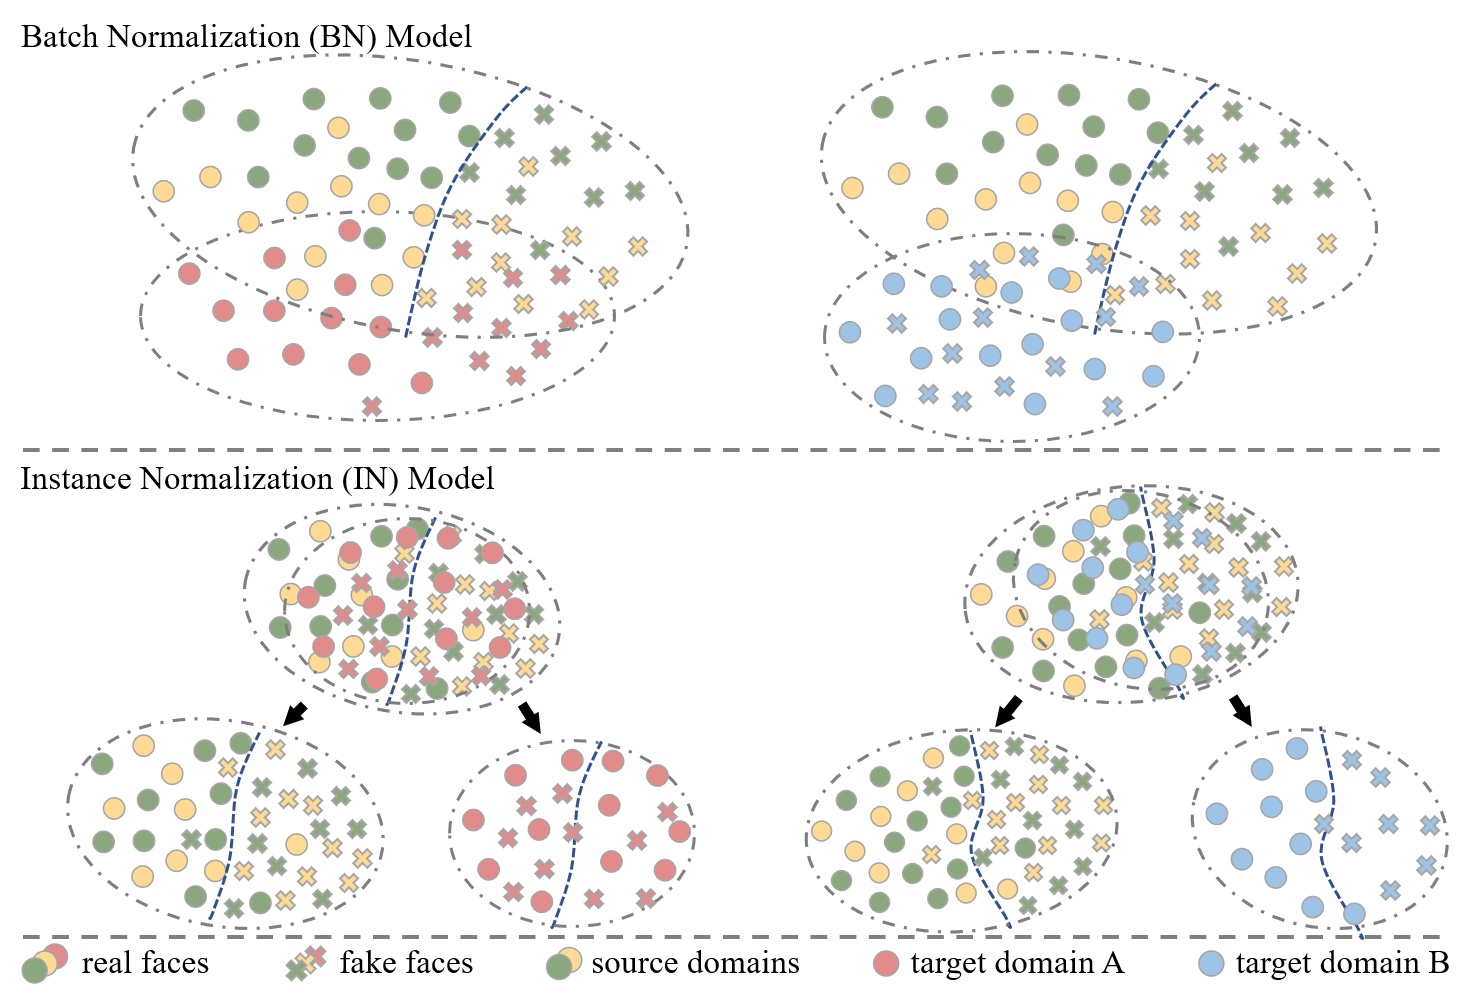
\includegraphics[width=\linewidth]{img/illustrate.png}
\end{frame}

\begin{frame}{Objective: Domains shift}
    \begin{figure}[htbp]
        \centering
        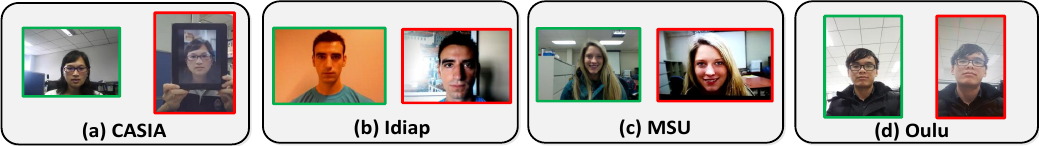
\includegraphics[width=0.9\textwidth]{img/datasets.png}
        \caption{Samples from CASIA-MFSD, Idiap, MSU, and Oulu datasets exhibiting severe domain shifts.}
    \end{figure}
    \begin{itemize}
        \item The framework generalizes well across previously unseen domains by remaining invariant to illumination and background variations.
        \item \textbf{Asymmetric class assumption}:
        \begin{itemize}
            \item \textit{Live}: Compact physiological similarity.
            \item \textit{Spoofs}: Highly heterogeneous.
        \end{itemize}
    \end{itemize}
\end{frame}


\begin{frame}{ANRL framework overview}
    \begin{figure}
        \centering
        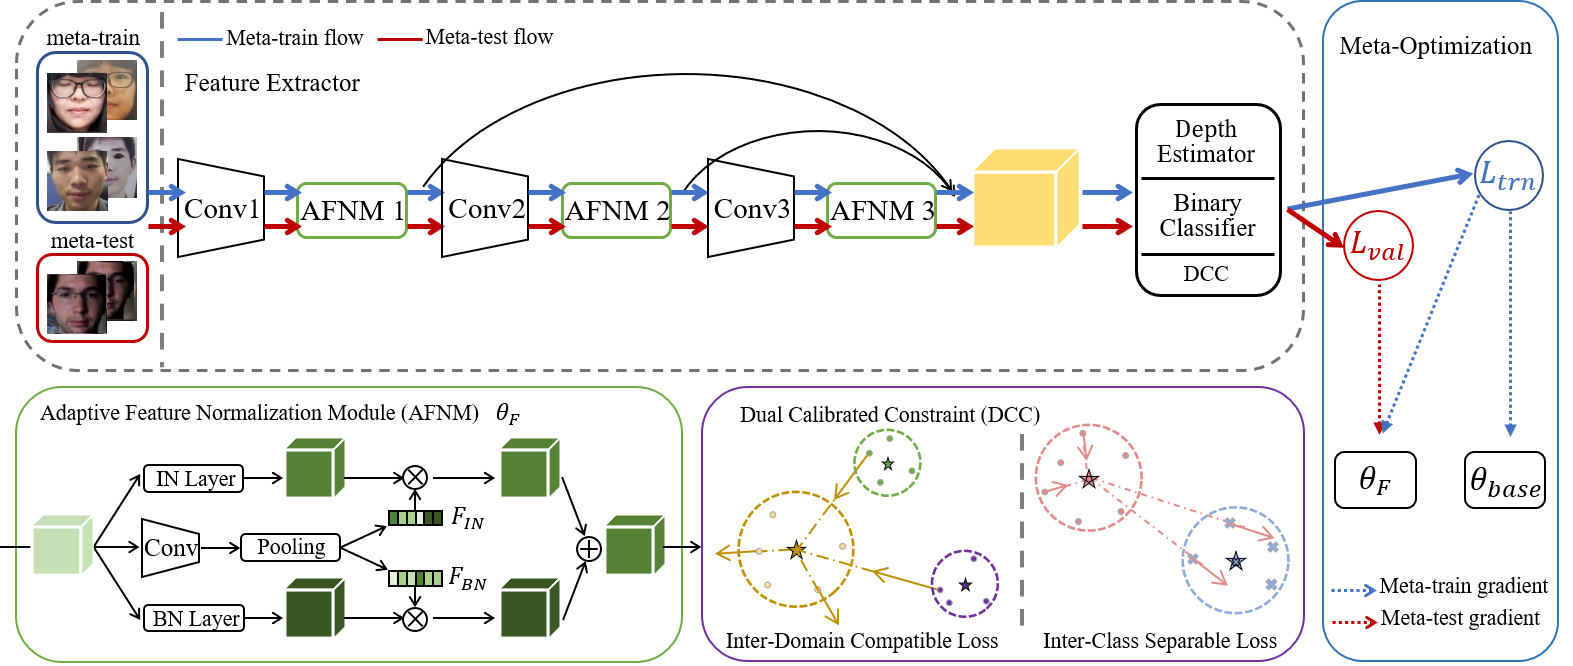
\includegraphics[width=\textwidth,height=0.85\textheight,keepaspectratio]{img/framework.png}
    \end{figure}
\end{frame}

\begin{frame}{Adaptive feature normalization module (AFNM)}
    \vspace{-1.0em}
    \begin{columns}[T]
        \begin{column}{0.4\textwidth}
            \small
            \textbf{Dual calibrated constraints (DCC)}:
            \begin{itemize}
                \item \textbf{IDC}: Minimizes domain bias by mixing source domains. $\mathcal{L}_{IDC} = \sum_{k=1}^{K} (D_{dd}^k - D_{sd}^k)$
                \item \textbf{ICS}: Compacts real faces, scatters fakes. $\mathcal{L}_{ICS} = D_{rr} - D_{rf} - D_{fr}$
            \end{itemize}
            \textbf{Note}: 
            \begin{itemize}
                \item IDC: reduce BN corruption due to domain bias
                \item $D_{ff}$ is not included because presentation attacks are diverse.
            \end{itemize}
        \end{column}
        \begin{column}{0.6\textwidth}
            \textbf{AFNM mechanism}:
            \begin{itemize}
                \item \textbf{Dual normalizations}: BN and IN applied to input $X$.
                \item \textbf{Attention factors $\alpha_c$}: Computed via pooling and FC layers over $X$.
                \item \textbf{Adaptive fusion}: $Y_c = \alpha_c X_{c}^{BN} + (1 - \alpha_c) X_{c}^{IN}$.
            \end{itemize}

            \vspace{0.5em}
            \begin{figure}
                \scalebox{0.6}{
                \begin{tikzpicture}[
                    node distance=1.0cm and 1.5cm,
                    auto, >=stealth, scale=0.9, every node/.style={transform shape},
                    block/.style={rectangle, draw, fill=blue!10, text centered, rounded corners, minimum height=0.6cm, thick, font=\small},
                    opcircle/.style={circle, draw, fill=gray!20, text centered, inner sep=1pt, thick, font=\small},
                    oprect/.style={rectangle, draw, fill=gray!20, text centered, rounded corners, inner sep=2pt, thick, font=\small},
                    line/.style={draw, -stealth, thick}
                ]
                    \node [block] (input) {Input $X$};
                    \node [block, above right=0.3cm and 2.5cm of input] (bn) {BN ($X^{BN}$)};
                    \node [block, right=2.5cm of input, text width=2.5cm, align=center] (stat) {Pool ($S$), FC,\\ \textbf{Soft attention}};
                    \node [block, below right=0.3cm and 2.5cm of input] (in) {IN ($X^{IN}$)};
                    \node [oprect, right=2.0cm of bn] (mult1) {$\times \alpha$};
                    \node [oprect, right=2.0cm of in] (mult2) {$\times (1-\alpha)$};
                    \path (mult1) -- coordinate (mid) (mult2);
                    \node [opcircle, right=1.0cm of mid] (add) {$+$};
                    \node [block, right=0.8cm of add] (output) {Output $Y$};

                    \draw [line] (input.east) -- ++(0.3,0) |- (bn.west);
                    \draw [line] (input.east) -- (stat.west);
                    \draw [line] (input.east) -- ++(0.3,0) |- (in.west);
                    \draw [line] (stat.east) -| node[pos=0.75, right, font=\footnotesize] {} (mult1.south);
                    \draw [line] (stat.east) -| node[pos=0.75, right, font=\footnotesize] {} (mult2.north);
                    \draw [line] (bn.east) -- (mult1.west);
                    \draw [line] (in.east) -- (mult2.west);
                    \draw [line] (mult1.south east) -- (add.north west);
                    \draw [line] (mult2.north east) -- (add.south west);
                    \draw [line] (add.east) -- (output.west);
                \end{tikzpicture}
                }
            \end{figure}
        \end{column}
    \end{columns}
\end{frame}

\begin{frame}[shrink=10]{AFNM: In-depth analysis}
    \footnotesize
    \textbf{Core intuition}: 
    \begin{itemize}
        \item \textbf{BN} (\textit{Batch Normalization}): Preserves discriminative cues but is fragile to domain shifts.
        \item \textbf{IN} (\textit{Instance Normalization}): Eliminates domain style but may discard attack artifacts.
    \end{itemize}
    \vspace{0.2em}
    \textbf{Mathematical formulation}:
    \begin{itemize}
        \item \textbf{Statistic extraction}: Global average pooling captures spatial information:
        \vspace{-0.5em}
        \begin{equation*}
            S_c = F_{gp}(X) = \frac{1}{H \times W} \sum_{i=1}^{H} \sum_{j=1}^{W} X_c(i,j)
        \end{equation*}
        \item \textbf{Fully-connected layer}: A fully connected layer learns a compact representation $Z$:
        \vspace{-0.5em}
        \begin{equation*}
            Z = F_{fc}(S) = \delta(WS)
        \end{equation*}
        \item \textbf{Adaptive fusion}: Soft attention derives sample-wise channel weights $\alpha_c$:
        \vspace{-0.5em}
        \begin{equation*}
            \alpha_c = \frac{\sigma(W_B Z)_c}{\sigma(W_B Z)_c + \sigma(W_I Z)_c}, \quad Y_c = \alpha_c X_{c}^{BN} + (1 - \alpha_c) X_{c}^{IN}
        \end{equation*}
    \end{itemize}
\end{frame}


\begin{frame}[shrink=2]{Base model}
    3 primary components: a Feature Extractor ($Ext$), a Binary Classifier ($BC$), and an auxiliary Depth Estimator ($Dep$).
    
    \begin{columns}[T]
        \begin{column}{0.65\textwidth}
            \textbf{1. Binary classification ($\mathcal{L}_{Cls}$):}
            \begin{itemize}
                \small
                \item Optimized using standard cross-entropy loss:
                \vspace{-0.5em}
                \begin{equation*}
                    \mathcal{L}_{Cls} = -\sum_{(x_i,y_i)} y_i \log(BC(Ext(x_i)))
                \end{equation*}
                \item Solely optimizing $\mathcal{L}_{Cls}$ often causes overfitting to domain-specific 2D textures.
            \end{itemize}
            
            \vspace{0.5em}
            \textbf{2. Depth estimation ($\mathcal{L}_{Dep}$):}
            \begin{itemize}
                \small
                \item Prevents converging on superficial 2D artifacts. Live faces possess 3D depth, whereas spoofing attacks are flat.
                \vspace{-0.5em}
                \begin{equation*}
                    \mathcal{L}_{Dep} = \sum_{(x_i,dep_i)} \left\| Dep(Ext(x_i)) - dep_i \right\|_{2}^{2}
                \end{equation*}
            \end{itemize}
        \end{column}
        \begin{column}{0.35\textwidth}
            \vspace{2.5em}
            \begin{figure}
                \centering
                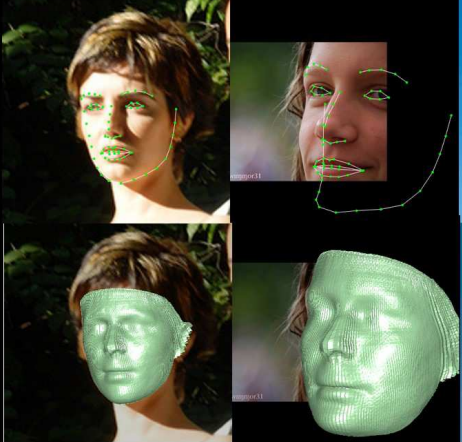
\includegraphics[width=\textwidth]{img/depthmap.png}
                \caption{\scriptsize Pseudo-depth map $dep_i$: 3D map for live faces via PRNet \cite{feng2018joint}, flat zero-map for spoofs.}
            \end{figure}
        \end{column}
    \end{columns}
\end{frame}

\begin{frame}{Optimization strategy: Meta learning}
    \vspace{-0.5em}
    \begin{algorithm}[H]
        \caption{The optimization strategy of ANRL}
        \label{optimization_strategy}
        \scriptsize
        \begin{algorithmic}[1]
            \Require $N$ source domains $\mathcal{D} = [D_1,D_2,\dots,D_N]$
            \State Initialize parameters $\theta_{F}$ of AFNM and parameters $\theta_{base}$ of other modules.
            \State Determine learning rates $\beta_{1}$, $\beta_{2}$ and hyper-parameters $\lambda_1$, $\lambda_2$.
            \State Shuffle all samples from different domains.
            \For{$t = 1$ to $N_{epoch}$}
                \State \textbf{Normal train}: Sample batch in $\mathcal{D}$.
                \State $\mathcal{L}_{base}(\theta_{base},\theta_{F}) = \sum_{\mathcal{D}} \mathcal{L}_{Cls} + \mathcal{L}_{Dep}$.
                \State $\theta_{base} \leftarrow \theta_{base} - \beta_1 \nabla_{\theta_{base}} \mathcal{L}_{base}(\theta_{base},\theta_{F})$.
                
                \State \textbf{Meta-train}: Sample batch in $D_{trn}$.
                \State $\mathcal{L}_{trn}(\theta_{base},\theta_{F}) = \mathcal{L}_{Cls(D_{trn})} + \mathcal{L}_{Dep(D_{trn})} + \lambda_1 \mathcal{L}_{IDC(D_{trn})} + \lambda_2 \mathcal{L}_{ICS(D_{trn})}$.
                \State $\theta_{F}' = \theta_{F} - \beta_1 \nabla_{\theta_{F}} \mathcal{L}_{trn}(\theta_{base},\theta_{F})$.
                
                \State \textbf{Meta-test}: Sample batch in $D_{val}$.
                \State $\mathcal{L}_{val}(\theta_{base},\theta_{F}') = \mathcal{L}_{Cls(D_{val})} + \mathcal{L}_{Dep(D_{val})} + \lambda_1 \mathcal{L}_{IDC(D_{val})} + \lambda_2 \mathcal{L}_{ICS(D_{val})}$.
                
                \State \textbf{Meta-optimization}: Update AFNM using combined gradients:
                \State $\theta_{F} \leftarrow \theta_{F} - \beta_2 \nabla_{\theta_{F}} (\mathcal{L}_{trn}(\theta_{base},\theta_{F}) + \mathcal{L}_{val}(\theta_{base},\theta_{F}'))$.
            \EndFor
            \State \Return Model parameters $\theta_{F}$ and $\theta_{base}$.
        \end{algorithmic}
    \end{algorithm}
\end{frame}
